\chapter{Sequence Tagging}

\section{Part of Speech (PoS) Tagging}

\dfn{PoS Tagging}{
Assegnare dei tag per distinguere le varie parti di una frase.
}

\subsection{Perché studiare PoS?}

\qs{}{Perché studiare PoS?}

\begin{itemize}
  \item Text-to-Speech: la pronuncia di alcune parole cambia in base alla loro parte nel discorso. 
  \item Scrivere regexps: per cercare le frasi principali. 
  \item Input per un parser completo. 
  \item MT (Machine Translation): riordinare aggettivi e nomi nelle traduzioni. 
  \item Si potrebbe volere distinguere tra aggettivi o altre parti del discorso. 
  \item Si potrebbe voler studiare cambiamenti linguistici come la ceazione di nuove parole o shifting del significato.
\end{itemize}

\begin{figure}[h]
    \centering
    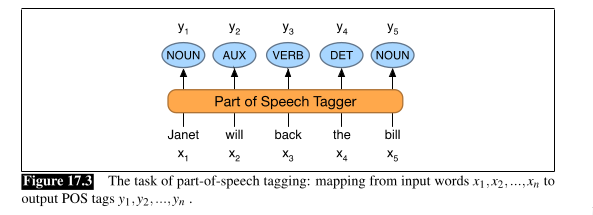
\includegraphics[scale=0.6]{02/PoS}
    \caption{Part of Speech Tagging.}
\end{figure}

\qs{}{Quanto è difficile il PoS Tagging?}

\begin{itemize}
  \item 85\% delle parole non sono ambigue. 
  \item 15\% delle parole sono ambigue e molto frequenti (il 60\% delle parole che si ascoltano sono ambigue).
\end{itemize}

\qs{}{Quanti tag sono corretti?}

\begin{itemize}
  \item Attualmente 97\%. 
  \item Una \textit{baseline} del 92\% è possibile con il metodo più banale:
    \begin{itemize}
      \item Si dà un tag a ogni parola con il suo significato più frequente. 
      \item Si dà un tag nome alle parole sconosciute.
    \end{itemize}
\end{itemize}

\begin{figure}[h]
    \centering
    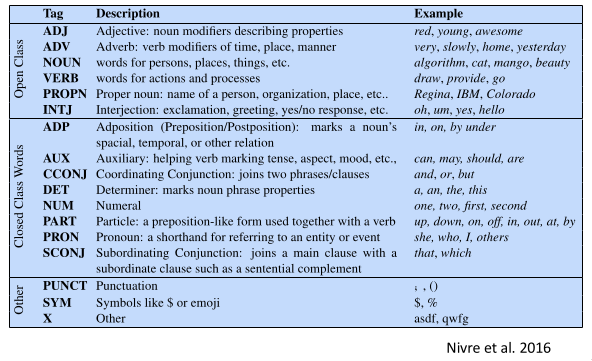
\includegraphics[scale=0.7]{02/tagset}
    \caption{Tagset.}
\end{figure}

\ex{\textit{Janet will back the bill}}{
\begin{itemize}
  \item Probabilità a parole: "will" è di solito un ausiliario.
  \item Identità delle parole adiacenti: "the" implica che la prossima parola probabilmente non è un verbo. 
  \item Morfologia e forma delle parole:
    \begin{itemize}
      \item Prefissi. 
      \item Suffissi. 
      \item Capitalizzazione.
    \end{itemize}
\end{itemize}
}

\paragraph{Algoritmi di supervised learning:}

\begin{itemize}
  \item Hidden Markov Models (programmazione dinamica). 
  \item Conditional Random Fields (CRF) / Maximum Entropy Markov Models (MEMM). 
  \item Natural Sequence Models (RNNs o transformers). 
  \item Large Language Models.
\end{itemize}

\subsection{Analisi Basata su Regole}

\paragraph{Idee di Base:}

\begin{enumerate}
  \item Assegnare tutti i possibili tags alle parole (analisi morfologica). 
  \item Rimuovere i tags in base a un \fancyglitter{insieme di regole}. 
  \item Solitamente più di 1000 regole scritte a mano (ma possono essere apprese automaticamente).
\end{enumerate}

\subsection{ENGTWOL Lexicon}

\begin{figure}[h]
    \centering
    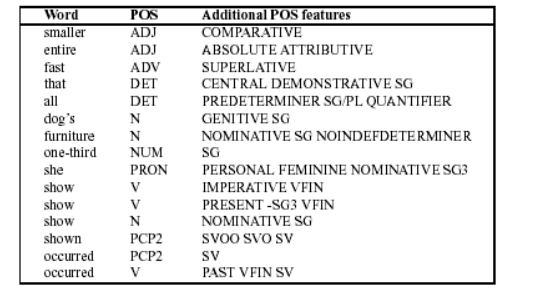
\includegraphics[scale=0.6]{02/eng.png}
    \caption{Esempio di ENGTWOL.}
\end{figure}

\begin{itemize}
  \item Utilizzare un analizzatore morfologico per ottenere tutte le parti del discorso. 
\begin{figure}[h]
    \centering
    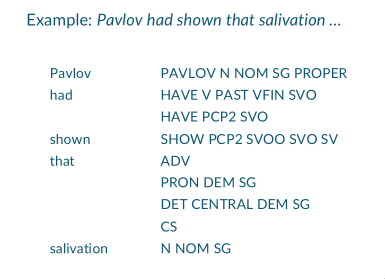
\includegraphics[scale=0.56]{02/eng2.png}
    \caption{Primo passaggio.}
\end{figure}
\item Si applicano i limiti. 
\begin{figure}[h]
    \centering
    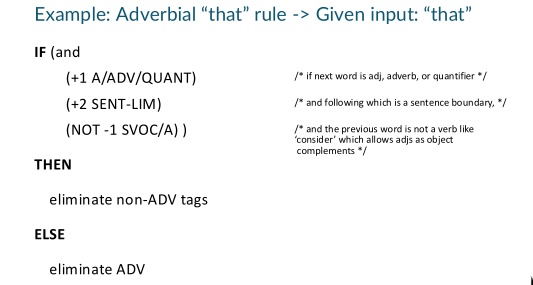
\includegraphics[scale=0.5]{02/eng3.png}
    \caption{Secondo passaggio.}
\end{figure}
\end{itemize}

\section{PoS Tagger Statistici}

\qs{}{Viene fornita una frase (un'osservazione o una sequenza di informazioni). Qual è la migliore sequenza di tags che corrisponde a questa sequenza di osservazioni?}

\paragraph{Vista probabilistica:}

\begin{itemize}
  \item Considera tutte le possibili sequenze di tags. 
  \item Di questo universo di sequenze viene scelta la sequenza più probabile.
\end{itemize}

\paragraph{Terminologia:}

\begin{itemize}
  \item \fancyglitter{Modelling}: fornire un modello formale. 
  \item \fancyglitter{Learning}: un algoritmo per impostare i parametri del modello. 
  \item \fancyglitter{Decoding}: un algoritmo per applicare il modello per calcolare risultati.
\end{itemize}

\subsection{HMM}

Si vuole modellare, di tutte le sequenze di $n$ tags $t_1...t_n$, la sequenza di tags tale che $P(t_1...t_n|w_1...w_n)$ è la maggiore. 

$$\hat{t}^n_1 = \text{argmax} P(t^n_1|w^n_1)$$

\nt{"\^" significa "la nostra stima del migliore". 

$argmax_x f(x)$ significa "la $x$ che massimizza $f(x)$."
}

\qs{}{Ma come si utilizza questa equazione?}

\paragraph{Inferenza Bayesiana:} si usa la regola di Bayes per trasformare quest'equazione in un insieme di probabilità che sono facilmente calcolabili.

\begin{figure}[h]
    \centering
    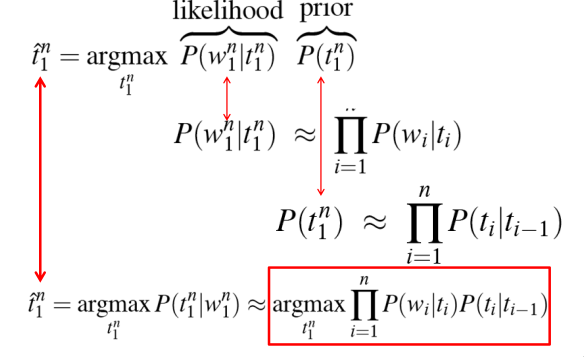
\includegraphics[scale=0.5]{02/bayes.png}
    \caption{Ipotesi di Markov, utilizzo dell'inferenza Bayesiana.}
\end{figure}

\nt{
  Nell'ipotesi di Markov sono presenti approssimazioni, per rendere il tutto più facile da calcolare.
}

\paragraph{Learning:}

\begin{itemize}
  \item PoS $\rightarrow$ PoS: 
    \begin{itemize}
      \item Si calcola la probabilità che una determinata parte di una frase ne preceda un'altra. 
      \item Esempio: $P(NN|DT) = \frac{C(DT,NN)}{C(DT)}$ è la probabilità che un articolo ($DT$) preceda un nome ($NN$).
      \item In generale $P(t_i|t_{i - 1}) = \frac{C(t_{i - 1}, t_i)}{C(t_{i - 1})}$, dove $C$ conta le occorrenze.  
    \end{itemize}
  \item PoS $\rightarrow$ World:
    \begin{itemize}
      \item Calcola la probabilità che una certa parola assuma una certa valenza (likehood, probabilità di verosomiglianza).
      \item Esempio: $P(is|VBZ) = \frac{C(VBZ, is)}{C(VBZ)}$, la probabità che un verbo alla terza persona presente (VBZ) sia $is$.
      \item $P(w_i|t_i) = \frac{C(t_i, w_i)}{C(t_i)}$.
    \end{itemize}
\end{itemize}

\begin{figure}[h]
    \centering
    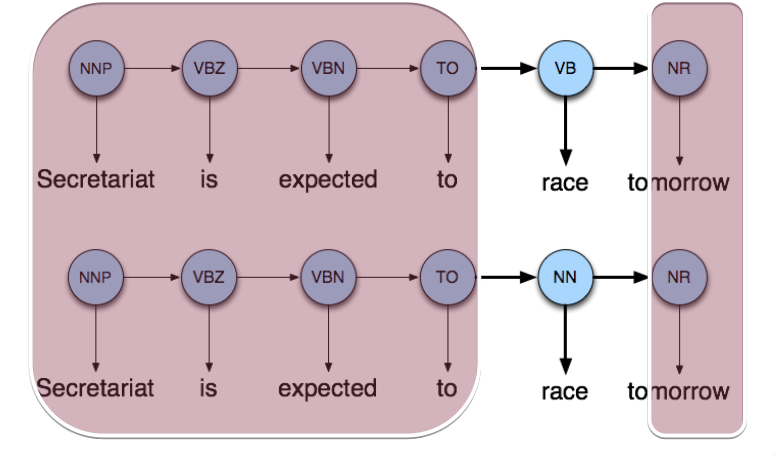
\includegraphics[scale=0.45]{02/dis.png}
    \caption{Disambiguare la parola "race".}
\end{figure}

\nt{Si va a calcolare la probabilità della parola diversa.}

\qs{}{Come si fa a fare il decoding?}

\begin{itemize}
  \item L'algoritmo banale (che non funziona) porta a considerare tutte le possibili sequenze e andare a prendere la probabilità maggiore. 
  \item Però con 30 tags e una frase di lunghezza media (20 parole) si hanno $30^{20}$ casi. 
\end{itemize}

\begin{figure}[h]
    \centering
    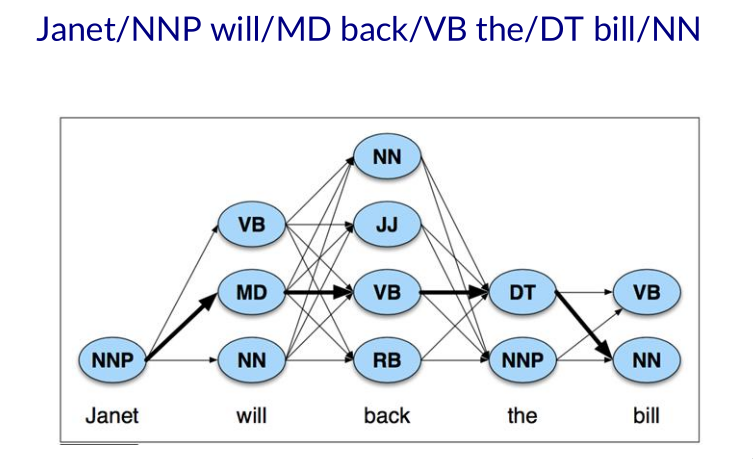
\includegraphics[scale=0.45]{02/janet.png}
    \caption{Tentativo di decoding.}
\end{figure}

\paragraph{Idee della programmazione dinamica:}

\begin{itemize}
  \item Si consideri una sequenza di stati (tag sequence) che termini con uno stato $j$ con un particolare tag $T$. 
  \item La probabilità che la tag sequence possa essere rotta in due parti: 
    \begin{itemize}
      \item La probabilità della migliore tag sequence attraverso $j - 1$. 
      \item Moltiplicata con la probabilità di transizione del tag alla fine della sequenza ($j-1$) rispetto a $T$
    \end{itemize}
\end{itemize}

\paragraph{Sommario di Viterbi:}

\begin{itemize}
  \item Crea una matrice:
    \begin{itemize}
      \item Con colonne corrispondenti agli input. 
      \item Con righe corrispondenti ai possibili stati (PoS\_Tag + $S_{ini} + S_{fin}$).
    \end{itemize}
  \item Si attraversa la matrice riempendo le colonne a destra con i valori immediatamente a sinistra. 
  \item Ogni cella della matrice, $v_i(j)$, rappresenta la probabilità che HMM sia nello stato $j$ dopo aver visto le prime $t$ parole e attraversato la sequenza di stati più probabile $q_1, \dots, q_{t-1}$. 
  \item $v_t(j) = max_{i=1}^N v_{t-1}(i) a_{i,j} b_j (o_t)$.
\end{itemize}
\pagebreak
\paragraph{Con i simboli:}

  \begin{itemize}
    \item $v_{t-1}(i)$: la probabilità della precedente iterazione dell'algoritmo di Viterbi. 
    \item $a_{i,j}$: la probabilità di transizione da un precedente stato $q_i$ allo stato corrente $q_j$. 
      \begin{figure}[h]
    \centering
    
\includegraphics[scale=0.25]{02/transition.png}
    \caption{Transition probability or something, idk.}
\end{figure}
\item $b_j(o_t)$: la likehood dello stato di osservazione del simbolo $o_t$ dato lo stato corrente $j$.
  \end{itemize}

\begin{figure}[h]
    \centering
    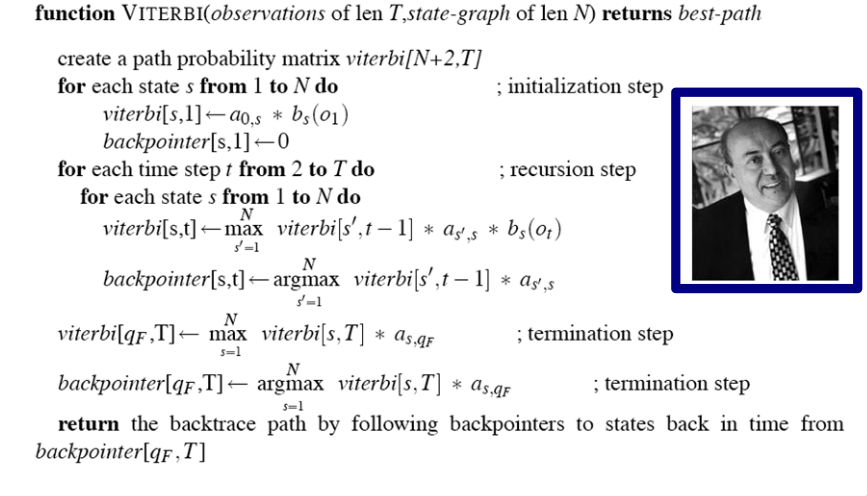
\includegraphics[scale=0.5]{02/viterbi.png}
    \caption{Algoritmo di Viterbi.}
\end{figure}

\nt{
  La chiave di programmazione dinamica è che abbiamo bisogno solo memorizzare il percorso prob MAX in ogni cella e non in tutti percorsi. 
}
\pagebreak
\paragraph{Un tag può non dipendere solo dal precedente, ma a volte ne servono due:}

\begin{figure}[h]
    \centering
    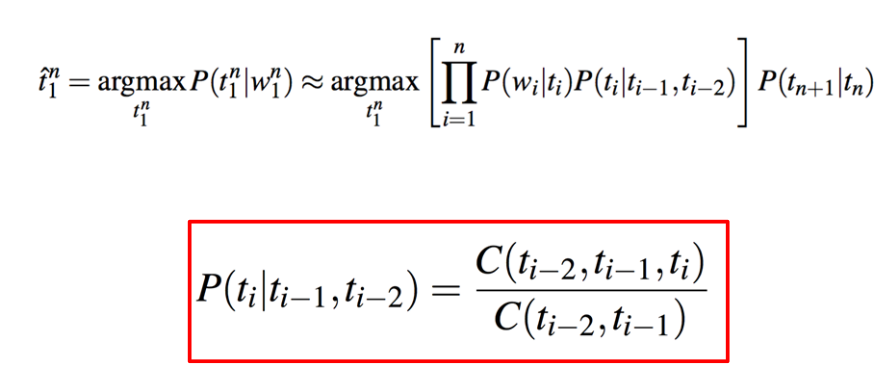
\includegraphics[scale=0.4]{02/due.png}
    \caption{Estensione a due tag.}
\end{figure}

\nt{Tuttavia molte coppie sono linguisticamente inesistenti e per ciò avranno probabilità 0. Il problema è la presenza di "falsi zeri" dovuti al fatto che si lavora con un dataset finito.}

\dfn{Sparsness}{
  La sparsness di una matrice si riferisce alla proporzione di elementi nulli rispetto al totale degli elementi della matrice. Una matrice è considerata sparsa (sparse matrix) se la maggior parte dei suoi elementi è uguale a zero:

$$S = \frac{\text{numero di elementi nulli}}{\text{numero totale di elementi}} = \frac{\text{\#zeri}}{m \times n}$$
}

\paragraph{Problemi degli HMM:}

\begin{itemize}
  \item Quanto il corpus sia grande o sparso.
  \item Come si può valutare la probabilità per parole sconosciute?
    \begin{itemize}
      \item Si possono usare alcune features: suffissi, capitalizzazione, etc.
    \end{itemize}
\end{itemize}

\subsection{MEMM e CRF}

Si può identificare un insieme di features su cui effettuare un modello probabilistico.

\begin{figure}[h]
    \centering
    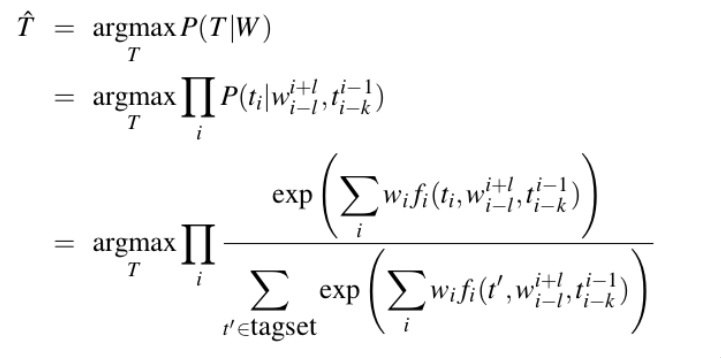
\includegraphics[scale=0.4]{02/MEMM.png}
    \caption{Il Maximum Entropy Markov Model (MEMM).}
\end{figure}

\paragraph{MEMM:}

\begin{itemize}
  \item Assegna le features alla parola stessa (non ha memoria). 
  \item Costruisce un classificatore per predirre il tag.
\end{itemize}

\paragraph{Apprendimento per MEMM:}

\begin{itemize}
  \item Regressione logistica multinomiale. 
  \item Viene scelto il parametro $w$ che massimizza la probabilità dell'etichetta $y$ nei dati riguardanti un osservazione $x$.
  \item Per via dell'utilizzo di pesi è più lento dei modelli generativi e ha un comportamento random.
  \item Per il decoding si può usare il viterbi con alcune correzioni.
\end{itemize}




\dfn{Conditional Random Fields (CRF)}{
  I CRF utilizzano features globali su un'intera sequenza. Sono modelli grafici molto complessi e potenti. 
}

\nt{In NLP sono catene lineari dove vengono accoppiate variabili ed etichette per tokens adiacenti.}

\clm{}{}{
  \begin{itemize}
    \item In un CRF la funzione $F$ mappa un'intera sequenza $X$ e un'intera sequenza di output $Y$ su un vettore di features. 
    \item A differenza del modello MEMM si calcola il peso sull'intera sequenza.
  \end{itemize}
}

\subsection{Tagging di Parole Sconosciute}

\paragraph{Possibili approcci per gestire parole sconosciute in HMM:}

\begin{itemize}
  \item Assumere che sono nomi. 
  \item Assumere una dstribuzione uniforme nel PoS. 
  \item Dizionari esterni. 
  \item Usare informazioni morfologiche (per esempio -are, -ere, -ire per i verbi in italiano). 
  \item Assumere che le parole sconosciute abbiano una probabilità di distribuzione simile alle parole che sono comparse nel training set.
\end{itemize}

\section{NER Tagging}

\dfn{Named Entity}{
  Una Named Entity è qualsiasi cosa che può essere indicata da un nome proprio. I 4 tags più comuni sono:
  \begin{itemize}
    \item PER (Person). 
    \item LOC (Location). 
    \item ORG (Organization). 
    \item GPE (Geo-Political Entity).
  \end{itemize}
}

\nt{Spesso sono multi-word.}

\dfn{NER Tagging}{
  Il task di name entity recognition (NER) consiste in: 
  \begin{enumerate}
    \item Trovare accorgimenti che costituiscono nomi propri. 
    \item Taggando il tipo di entità.
  \end{enumerate}
}

\qs{}{Perché si usa NER?}

\begin{itemize}
  \item \fancyglitter{Sentiment analysis}: i sentimenti del consumatore nei confronti di una particolare compagnia  persona. 
  \item \fancyglitter{Rispondere alle domande}: su un'entità. 
  \item \fancyglitter{Estrazione di informazioni}: riguardo un'entità da un testo.
\end{itemize}

\qs{}{Perché il NER è più difficile del PoS?}

\begin{itemize}
  \item Segmentation: bisogna dividere in segmenti che costituiscono le entità. 
  \item Ambiguita dei tipi (la stessa named entity può assumere significati diversi).
    
\end{itemize}

\dfn{BIO Tagging}{
  BIO (Begin Inside Out) è una tecnica per effettuare il NER Tagging. Si utilizza:
\begin{itemize}
  \item B per indicare che sta iniziando una named entity. 
  \item I per indicare che si è dentro una named entity. 
  \item O per indicare che si è fuori da una named entity.
\end{itemize}
}

\paragraph{Avendo $n$ tipi di entità diversi si avranno:}

\begin{itemize}
  \item 1 O tag. 
  \item $n$ B tags. 
  \item $n$ I tags. 
\end{itemize}

\nt{Quindi con $n$ entità si utilizzeranno $2n + 1$ tags diversi.}




